
\documentclass[8pt]{article}

\usepackage[utf8]{inputenc}

\usepackage{amsmath, bm}
\usepackage{graphicx}
\usepackage{amssymb}
\usepackage{float}
\usepackage{caption}
\usepackage{subcaption}
% set font size to 11pt

% set margin
\usepackage[margin=0.5in]{geometry}


\begin{document}

% insert pdf cover page here

\title{Lab report: 3A3 Supersonic Nozzle}
\author{lwp26}
\date{October 2023}
\maketitle

\section{Part 1 Convergent - divergent nozzle}

\begin{figure}[H]
    \centering
    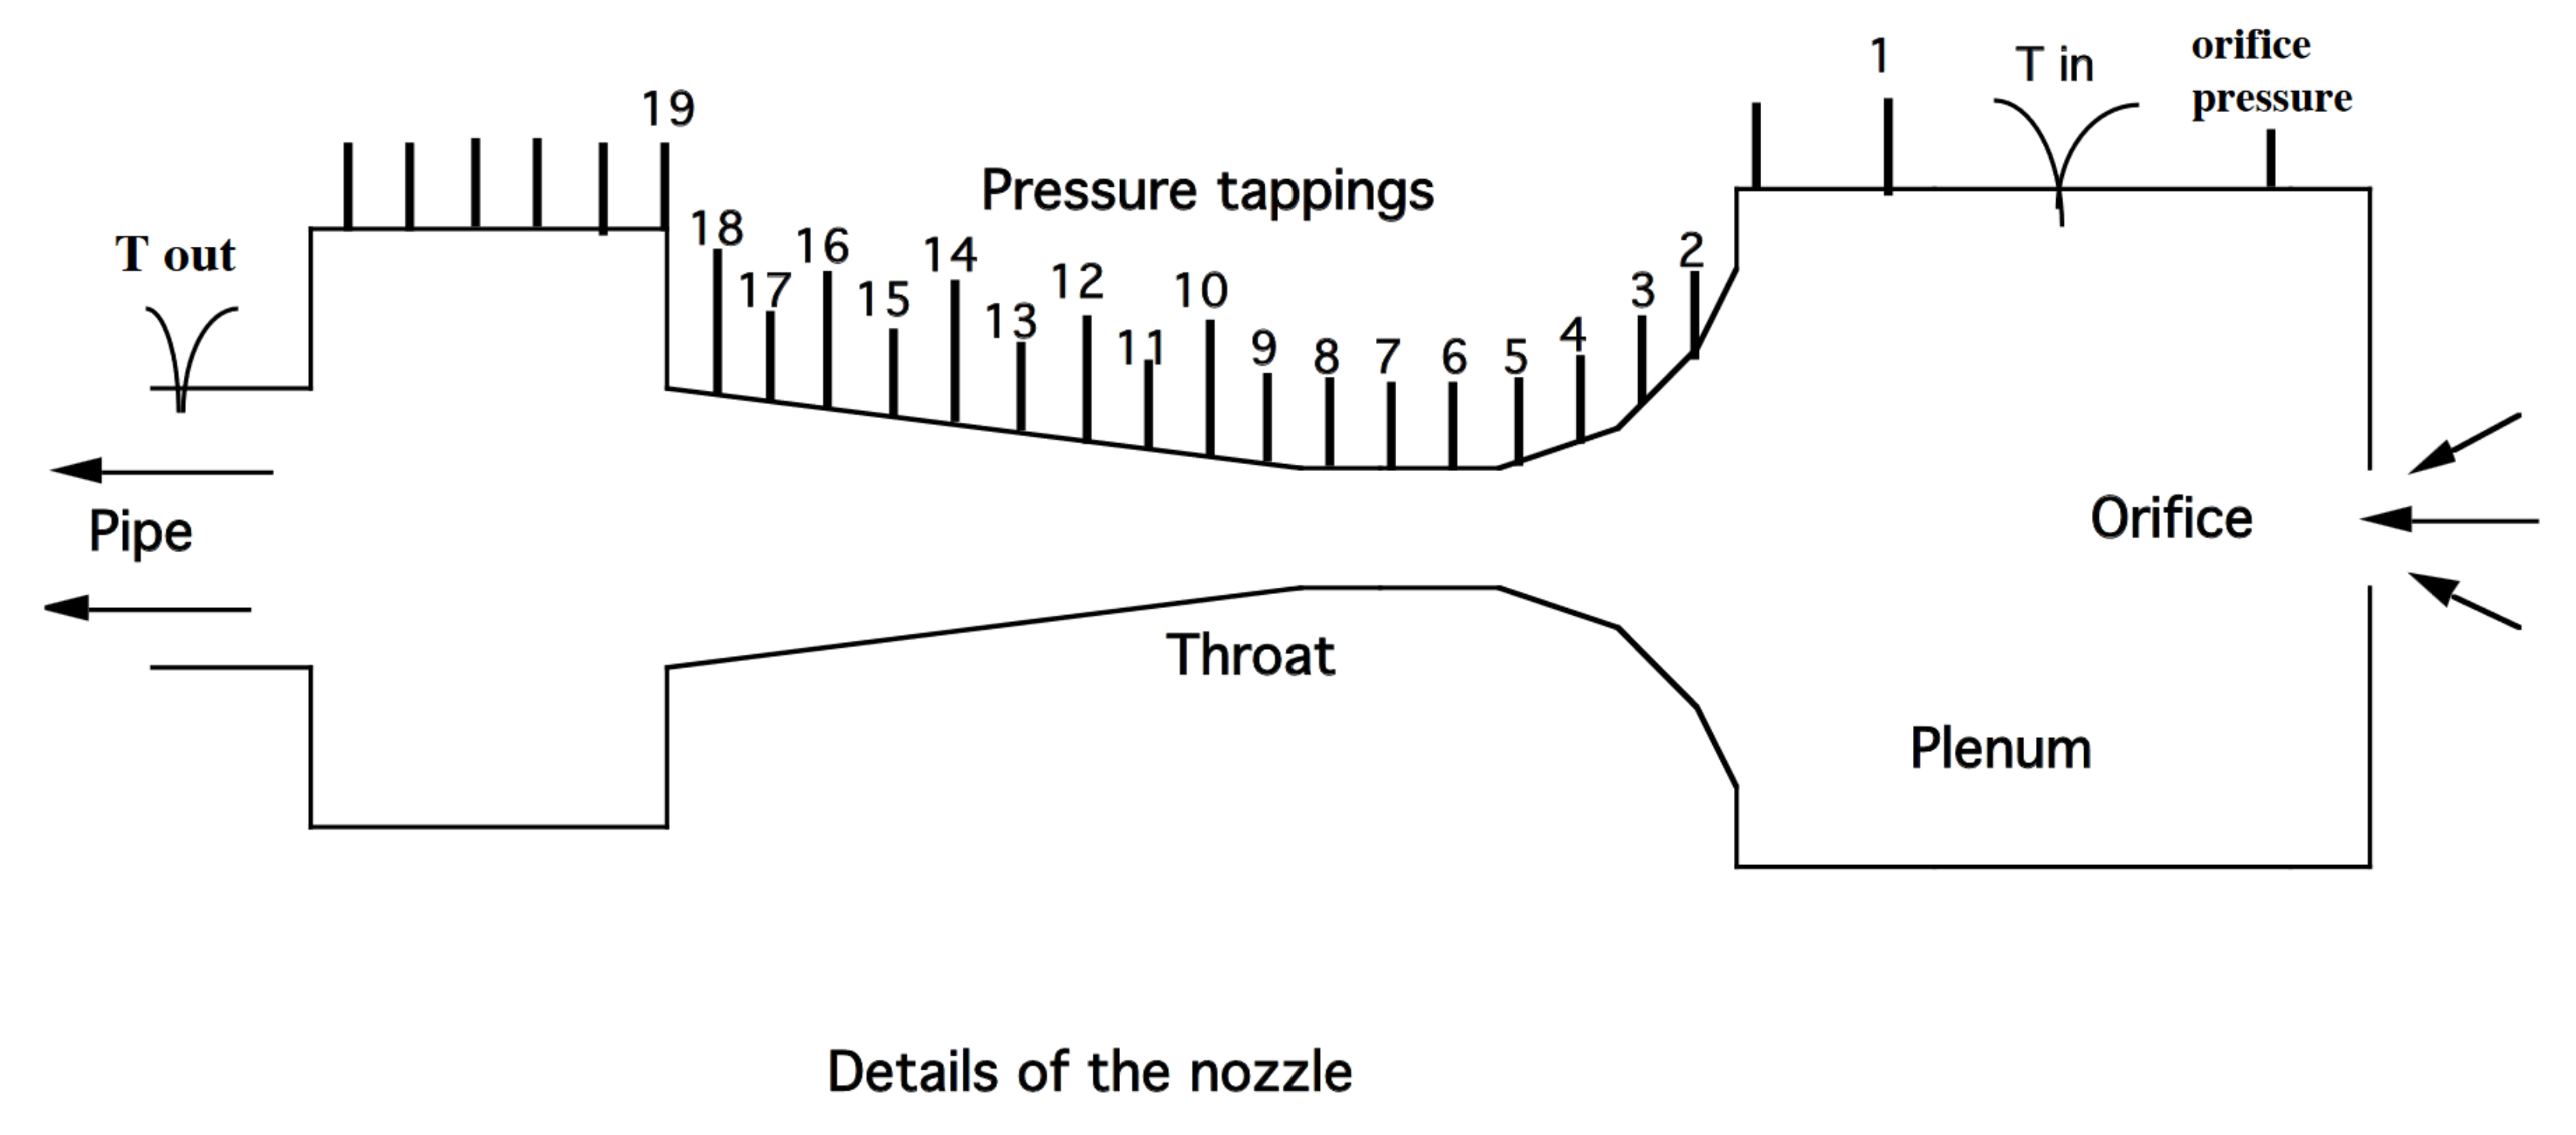
\includegraphics[width=0.8\textwidth]{small_nozzle_layout.png}
    \caption{Layout of Convergent - divergent nozzle}
    \label{fig:figure1}
\end{figure}

Orifice calibration: the diameter of the orifice is 17.47 mm. To a first approximation, assume that
\begin{itemize}
    \item The flow into the orifice is inviscid,
    \item the flow is slow enough to be treated as incompressible with density equal to that in the atmosphere upstream of the orifice (where the velocity is negligible),
    \item the velocity is uniform across the plane of the orifice,
    \item the pressure difference between the orifice plane and the upstream atmosphere is that measured on the
    water manometer
\end{itemize} 

To analyse the validity of the second assumption, consider the case of maximum flow, when the nozzil is choked upstream of the oriface, then its non-dimensional mass flow rate is given by the following equation.
\begin{equation}
    \frac{\dot{m}\sqrt{c_pT_0}}{p_0A^*} = 1.281
\end{equation}
From this, the non dimensional mass flow rate at the oriface can be calculated using the area ratio of the oriface to the nozzle throat.
The area of the throat was not known, however for demonstation purposes, the area of the oriface is taken to be twice that of the throat, and so the non-dimensional mass flow rate at the oriface is halved to $0.6405$.
At this point, the corresponding density ratio $\rho/\rho_0 = 0.9535 \approx 1$.
In reality the area of the oriface is much larger, and so this density ratio is a lower bound and so the assumption that the flow is incompressible is crude but sufficient for the purposes of this experiment.

The first and third assumptions are not valid as the flow is viscous and the velocity is not uniform across the plane of the oriface. However, they are accounted for by a discharge coefficient $C_d$, which is defined as the ratio of actual discharge to the ideal discharge.
The value of $C_d$ is constant at the high Reynolds numbers considered in this report.

With both the invicid and incompressible assumptions, the ideal flow rate through the orifice can be calculated using the pressure difference between the orifice plane and the upstream atmosphere is that measured on the
water manometer. By applying the Bernoulli equation from the upstream atmosphere (1) to the oriface plane (2),

\begin{equation}
    p_1 = p_2 + \frac{1}{2} \rho_a v_2^2
\end{equation}

Where $A$ and $v_2$ are the cross-sectional area, and velocity at the oriface. The theoretical mass flow rate through the oriface is then given by the following equation.
\begin{equation}
    \dot{m}_{ideal} = \rho_a A v_2 = \rho_a \left( \frac{\pi D^2}{4}\right) \sqrt{\frac{2(p_1-p_2)}{\rho_a}} \;\;\;\;\;\; \text{where} \;\;\;\;\;\ p_2 - p_1 = \rho_w g \Delta h
\end{equation}
Where $\rho_a$ is the density of air and $\rho_w$ is the density of water used for the manometer.
However, the actual flow rate through the orifice differs from the theoretical value as our assumptions are not valid.
This difference is characterised by the discharge coefficient $C_d$ which is defined as the ratio of the actual flow rate to the theoretical flow rate.
\begin{equation}
    \dot{m}_{actual} = C_d \dot{m}_{ideal}
\end{equation}
% https://arc.aiaa.org/doi/pdf/10.2514/6.2019-3651 ?
The discharge coefficient of the oriface is effectively constant over the range of high reynolds numbers considered in this experiment. 

\begin{figure}[H]
    \centering
    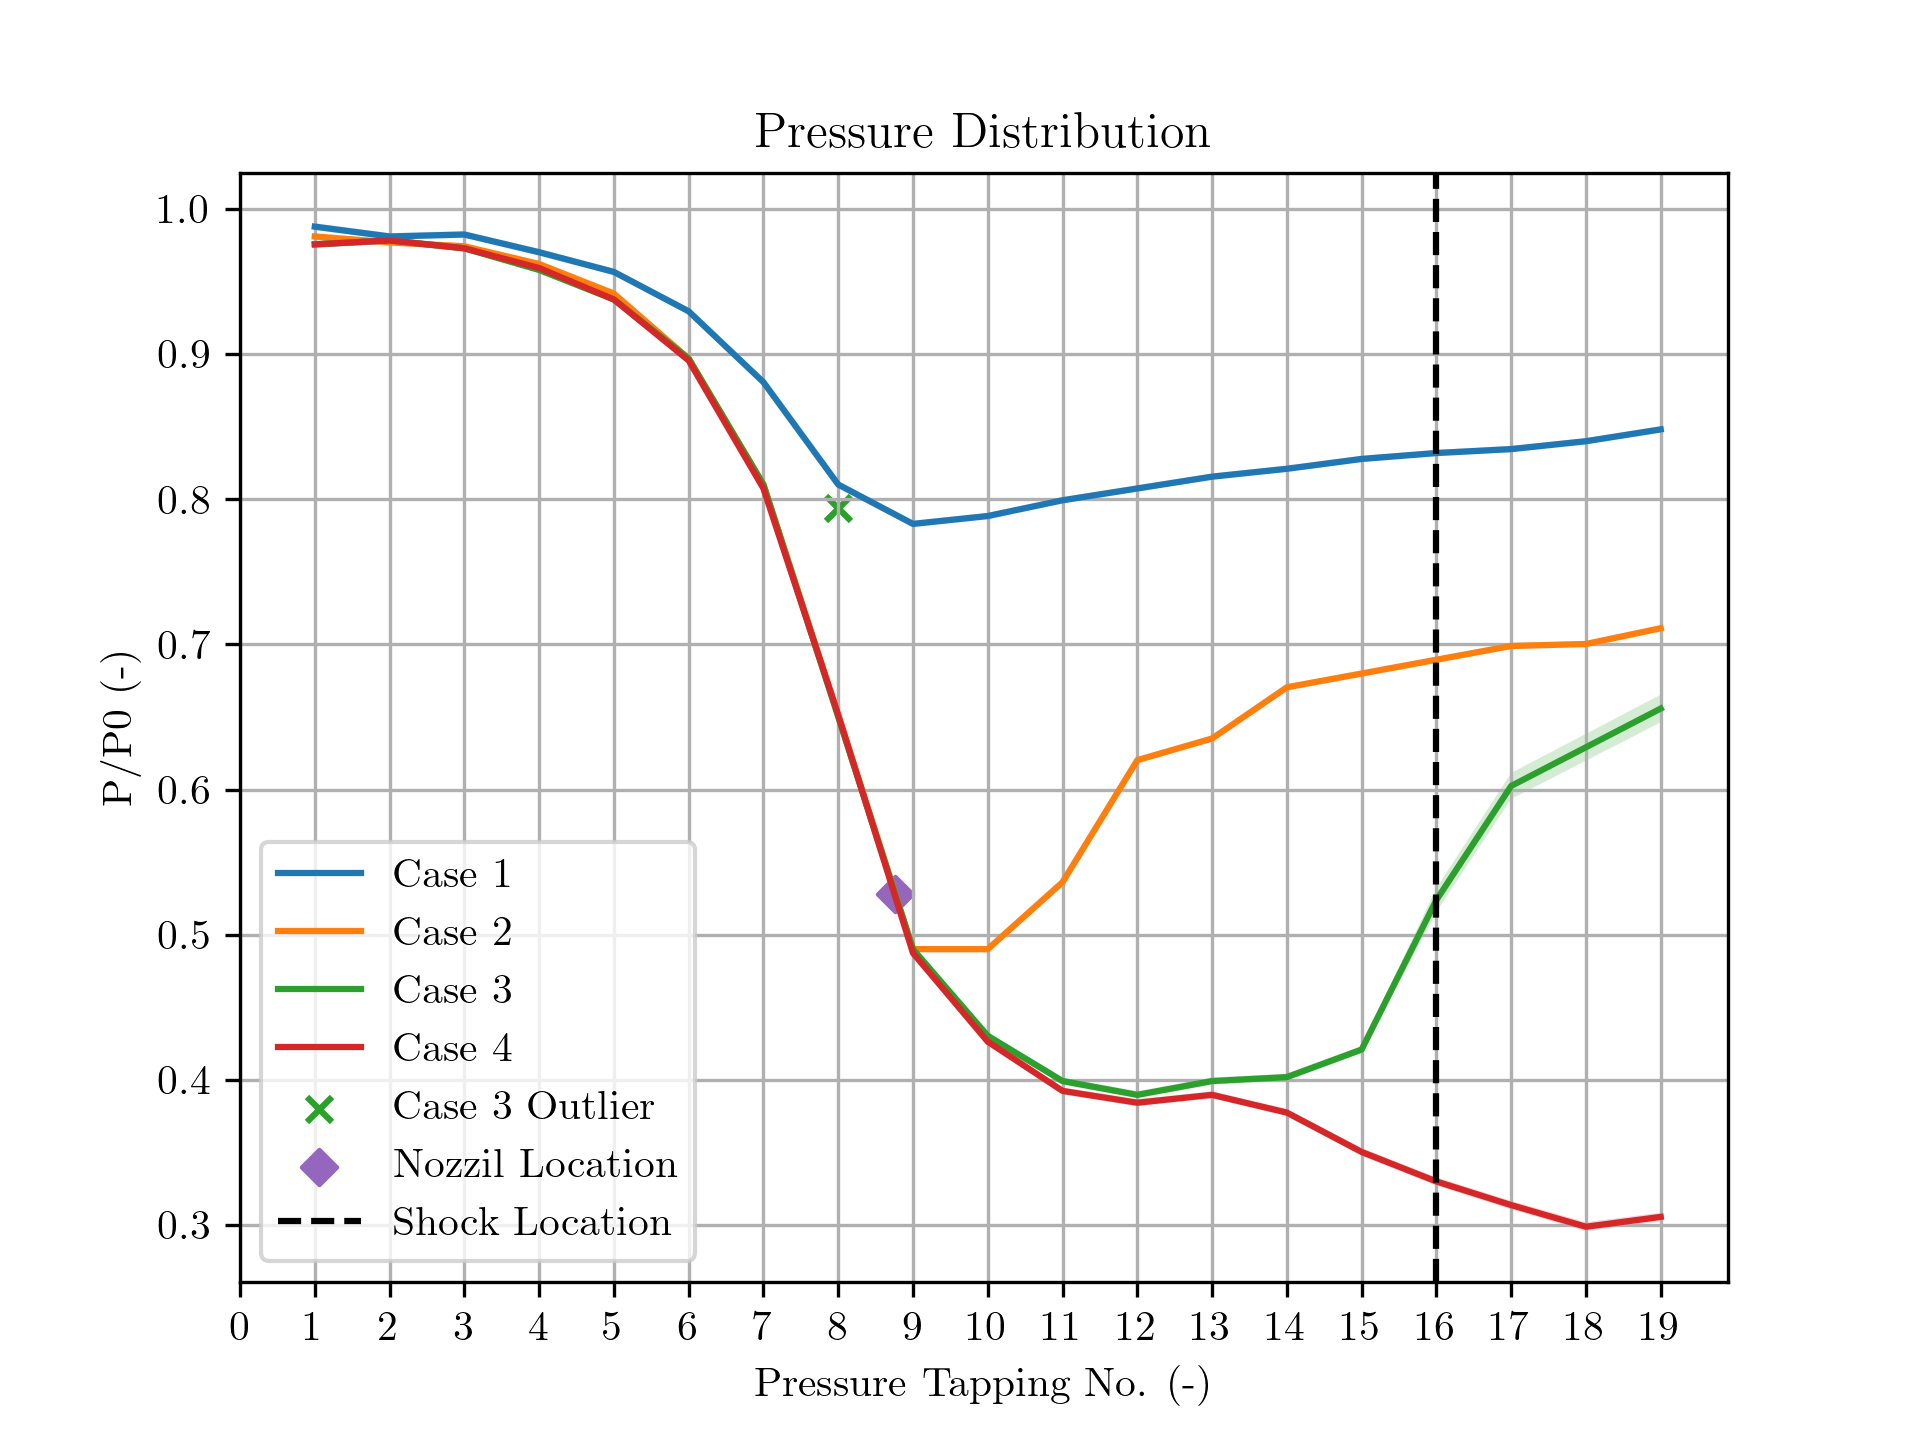
\includegraphics[width=0.8\textwidth]{pressure_ratio_distribution_corrected.png}
    \caption{Static pressure ratio distribution along the nozzle.}
    \label{fig:figure4}
\end{figure}

Figure \ref{fig:figure4} shows the static to stagnant pressure ratio distribution along the nozzle.
Case 2 is when the limiting choke condition is reached, and so the position of lowest pressure corresponds to the throat of the nozzle.
However, from the data on the graph this isnt a clear minimum, and so the throat position could be at position 9 or 10.
It will be taken to be at position 9 for the purposes of this report.

Using the assumption that the flow is adiabatic, and isentropic except for the shock wave in Case 3, which is accounted for later, the Mach number can be calculated from the static pressure ratio as follows:
% M2 = (rp ** - ((g-1)/g) - 1) * 2 / (g - 1)
\begin{equation}
    M = \frac{2}{\gamma - 1} \left[ \left( \frac{p}{p_0} \right) ^ {-\frac{\gamma - 1}{\gamma}} - 1 \right]
\end{equation}
This is plotted in figure \ref{fig:figure5} below.

\begin{figure}[H]
    \centering
    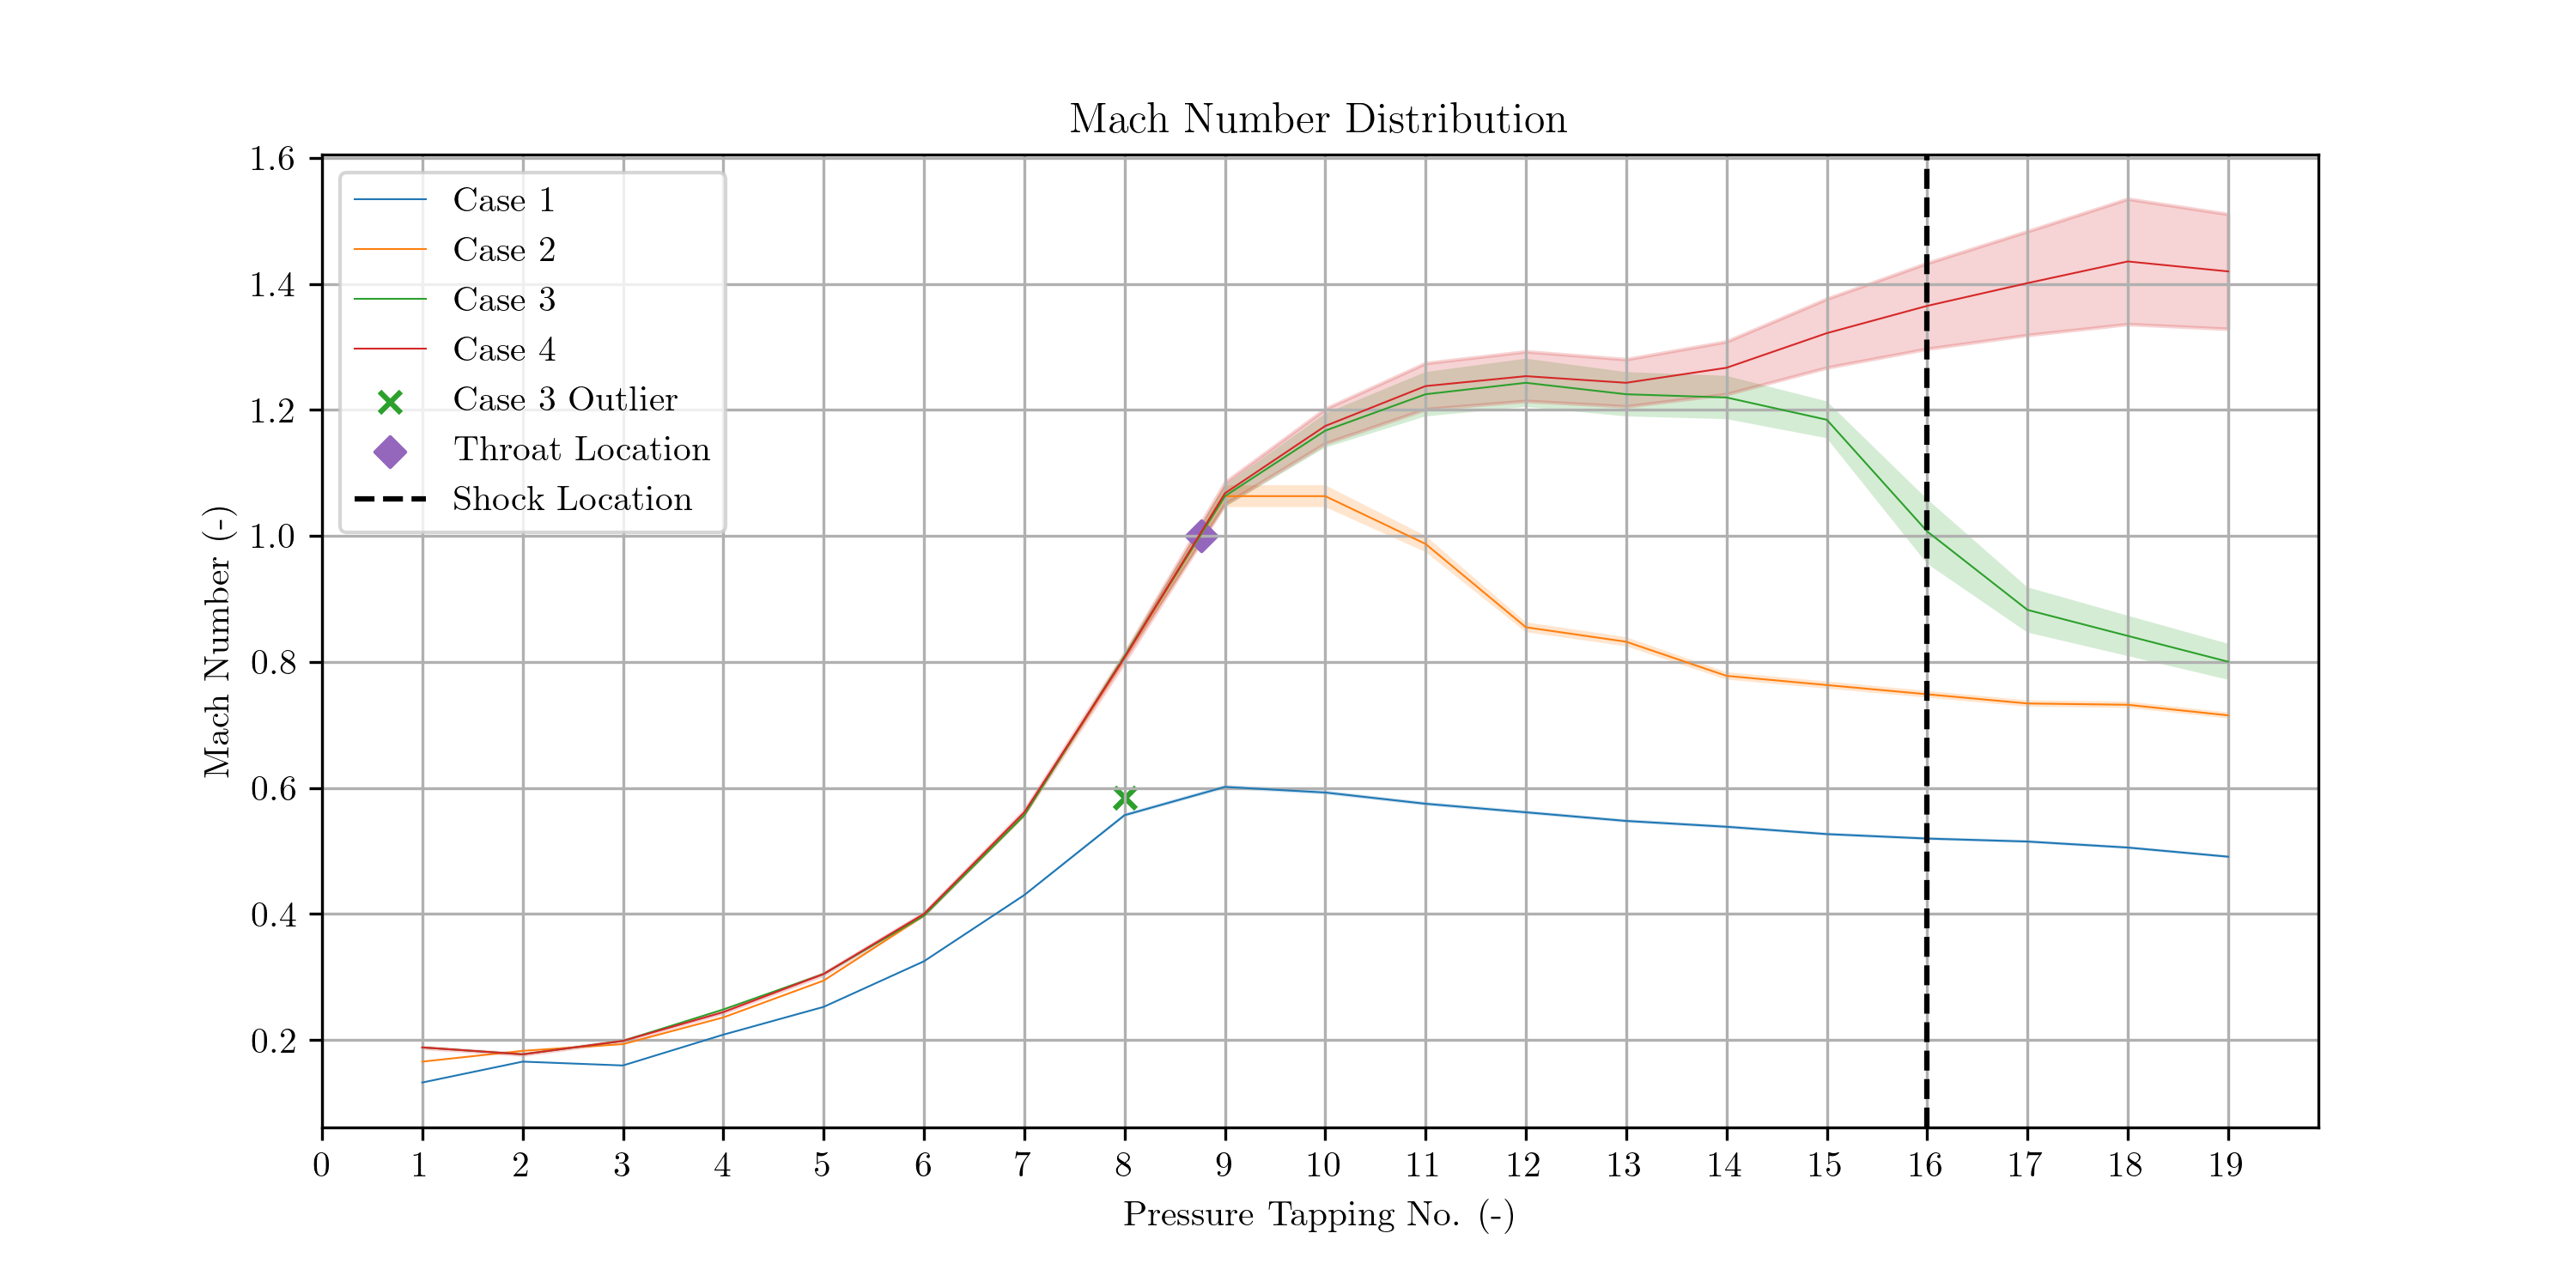
\includegraphics[width=0.8\textwidth]{mach_number_distribution_corrected.png}
    \caption{Figure 1}
    \label{fig:figure5}
\end{figure}
The plot of Mach number against position along the nozzle is shown below in figure \ref{fig:figure5}.

\begin{center}
    \captionof{table}{Exit and throat Mach numbers for each case.}
    \begin{tabular}{|c|c|c|}
    \hline 
    Case & Throat Mach No.  & Exit Mach No.\\
     & (-) & (-) \\
    \hline 
    1 & $0.602$ & $0.491$ \\
    2 & $1.063$ & $0.715$ \\
    4 & $1.068$ & $1.420$ \\
    \hline
    \end{tabular}
    \label{tab:1}
\end{center}

From looking at Case 3 where the shock wave is to be expected in the nozzle divergence, the Mach number increases from the throat to the exit of the nozzle then gradually decreases again.
The lack of sharp jump in pressure is mainly due to the fact that the measurements are taken at the wall where there are boundary layer effects.
The shock position is estimated to be at position 16.

% As a rough guess the shock in the core of the nozzle is assumed to be situated approximately at the axial position where $p/p_{0s}$ takes a value equal to $p/p_0$ for $M = 1$.
% what does this mean

The Mach number after the shock can be calculated from the Mach number before the shock, at 15, using the equation below:
% Ms from M
\begin{equation}
    M_s = \left( \frac{1 + \frac{\gamma - 1}{2} M^2}{\gamma M^2 - \frac{\gamma - 1}{2}} \right) ^ \frac{1}{2}
\end{equation}

Then the ratio of stagnant pressure ratios before and after the shock as a function of the Mach number before the shock is given by the following equation:
\begin{equation}
    \frac{p_{0s}}{p} = \left( \frac{\gamma + 1}{2} M^2 \right) ^ \frac{\gamma}{\gamma - 1} \left( \frac{2\gamma}{\gamma+1}M^2 - \frac{\gamma-1}{\gamma+1}\right) ^ \frac{1}{1 - \gamma}
\end{equation}
And so at position 16, before the shock $M = 1.036$ the stagnant pressure ratio is $p_{0s}/p = 0.999943 \approx 1$.
In figure \ref{fig:figure4} the static to stagnation pressure ratio of case 3, after the shock is divided by this value to give the correct static pressure ratio after the shock.
Figure \ref{fig:figure5} uses the corrected pressure ratios to calculate the Mach number after the shock using the same equation 5.


\begin{figure}[H]
    \centering
    \begin{subfigure}[t]{0.48\textwidth}
        \centering
        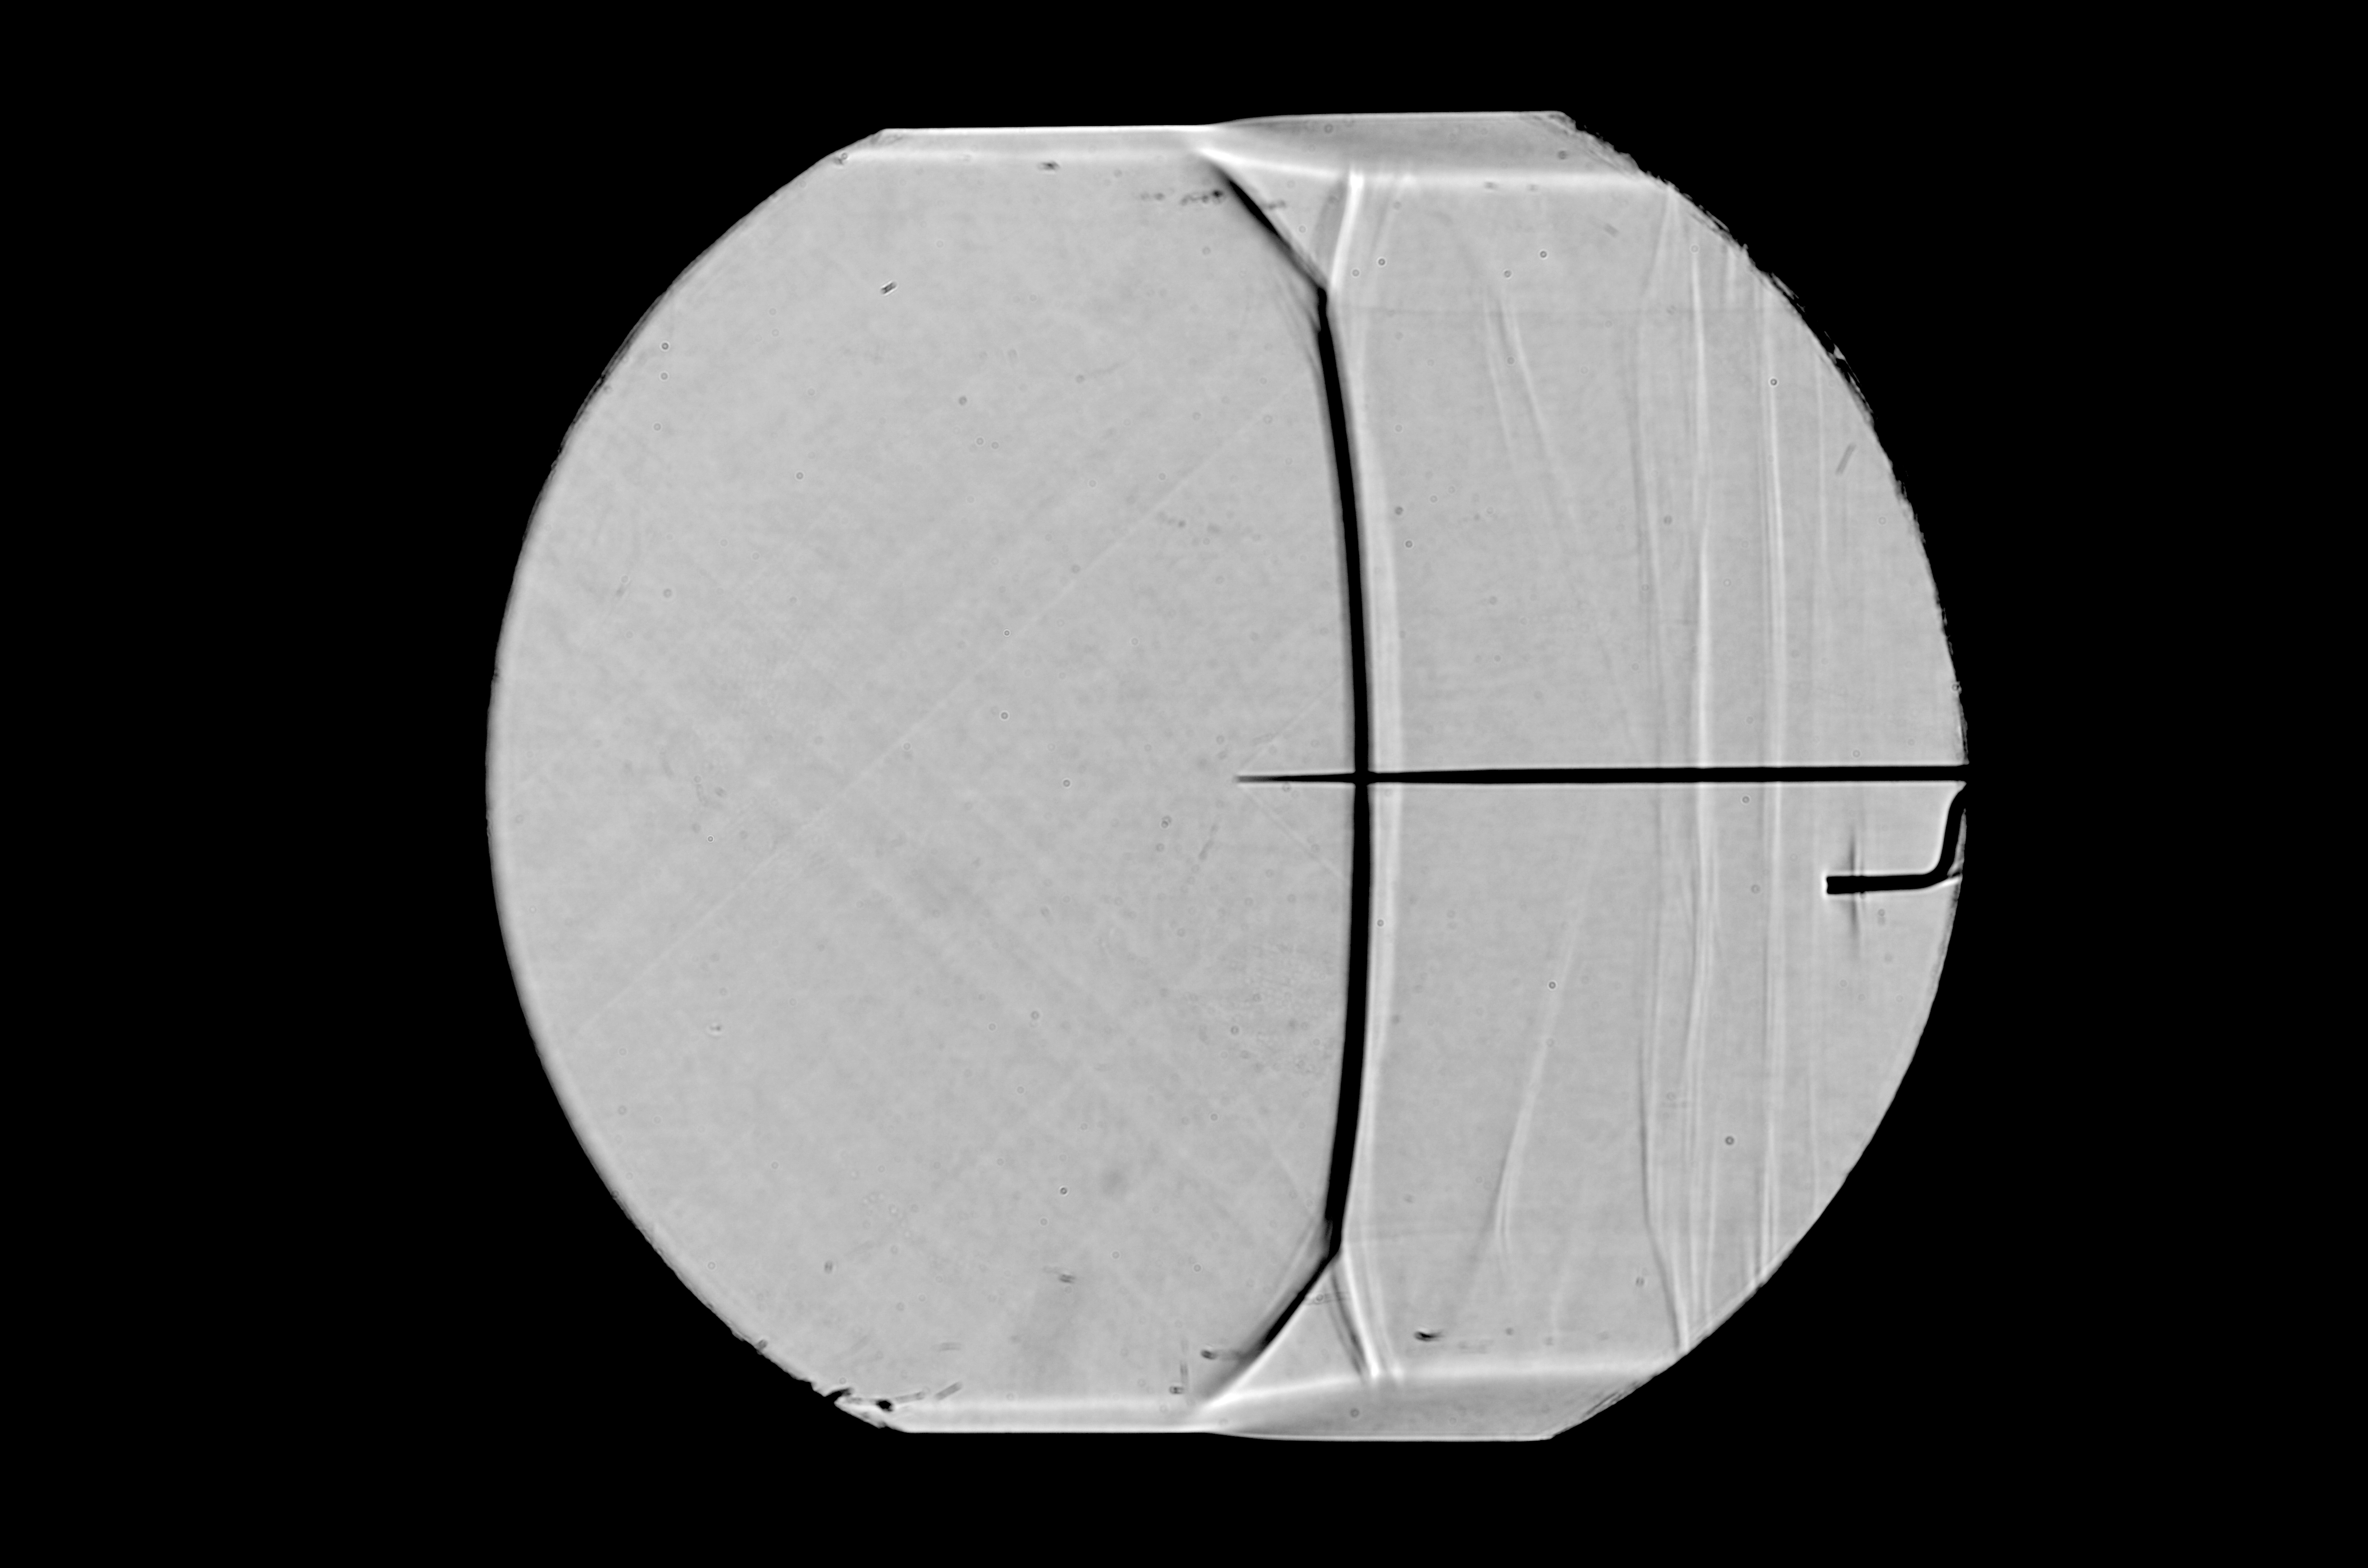
\includegraphics[width=1\textwidth]{starting_shock.jpg}
        \caption{Shock wave in working section before sensors}
        \label{fig:figure6}
    \end{subfigure}
    ~
    \begin{subfigure}[t]{0.48\textwidth}
        \centering
        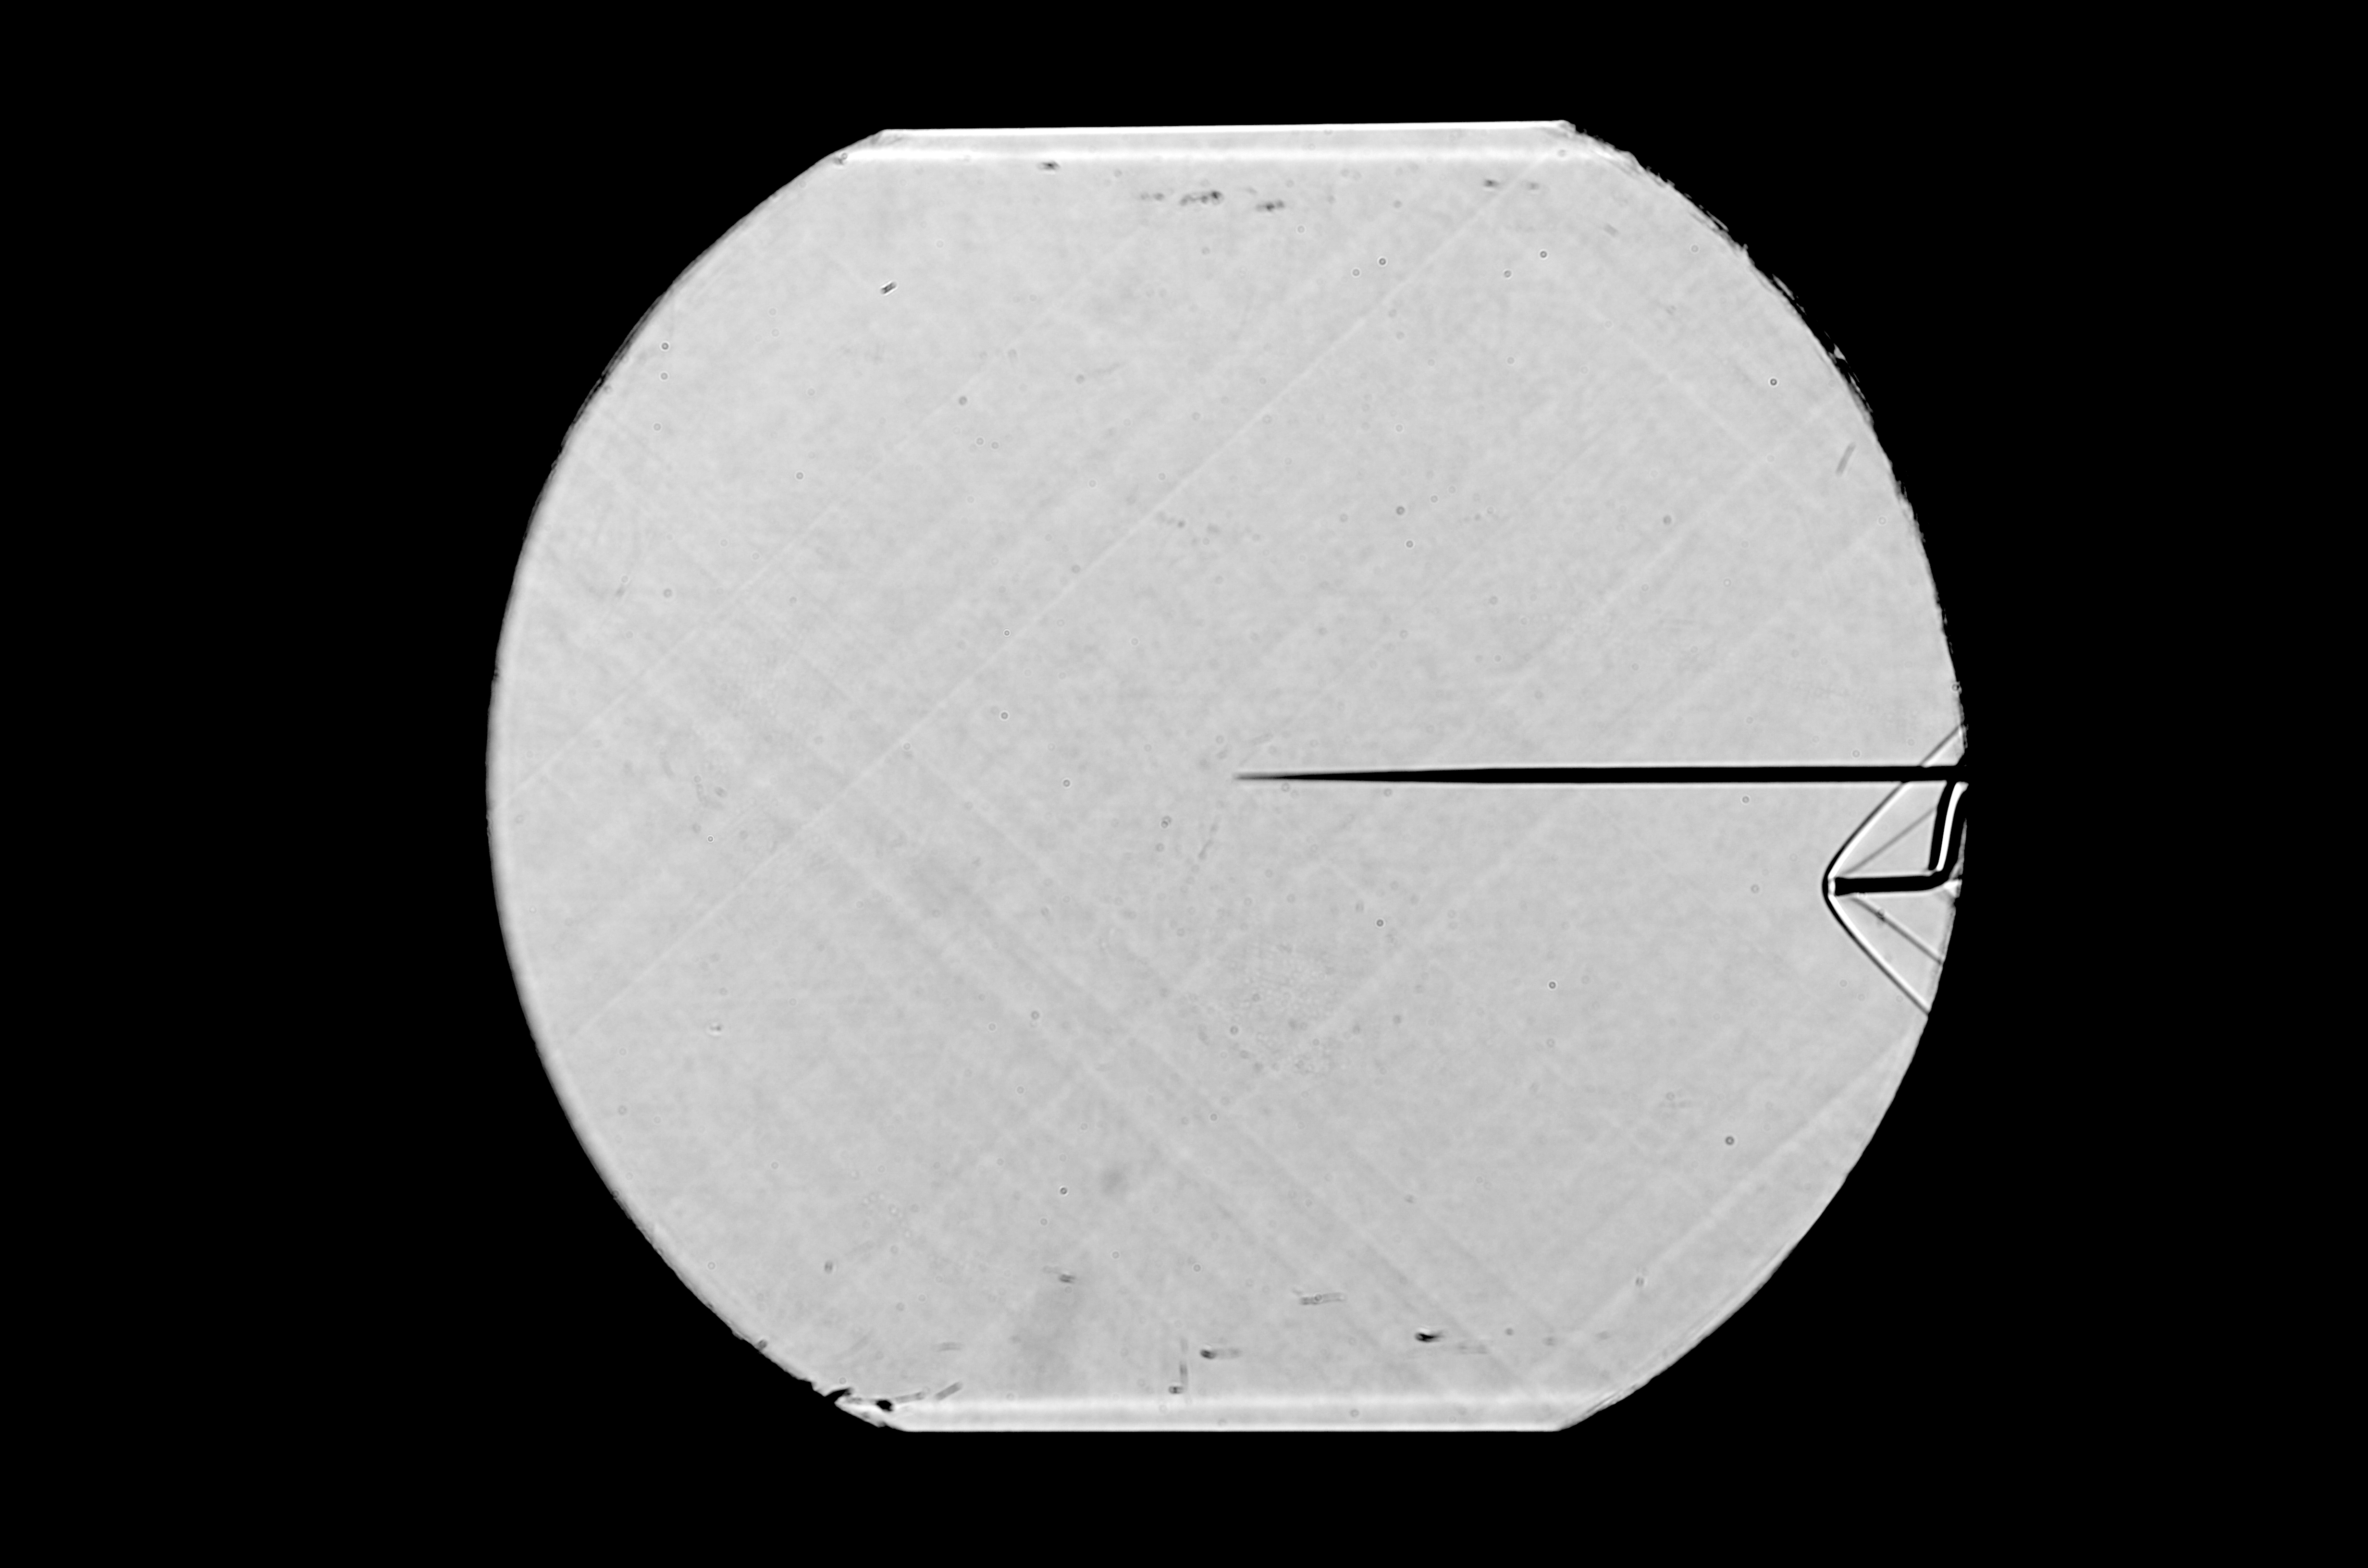
\includegraphics[width=1\textwidth]{working_state.jpg}
        \caption{Working state and bow shock of pitot probe}
        \label{fig:figure7}
    \end{subfigure}
    \caption{Shadowgraph images of the supersonic wind tunnel}
\end{figure}

Figure \ref{fig:figure6} shows the shock wave in the working section of the supersonic wind tunnel before the pressure sensors.
Shock waves of high density gradient are visible in the image from dark regions of the shadowgraph, where darker regions indicate stronger shock waves.
At the boundary layers at the top and bottom of the tunnel, the flow appears to travel through two shockwaves.
After the first shockwave the flow near the boundary layer is subsonic, but then must be accelerated again to supersonic speeds before the second, weaker shock.


\begin{figure}[H]
    \centering
    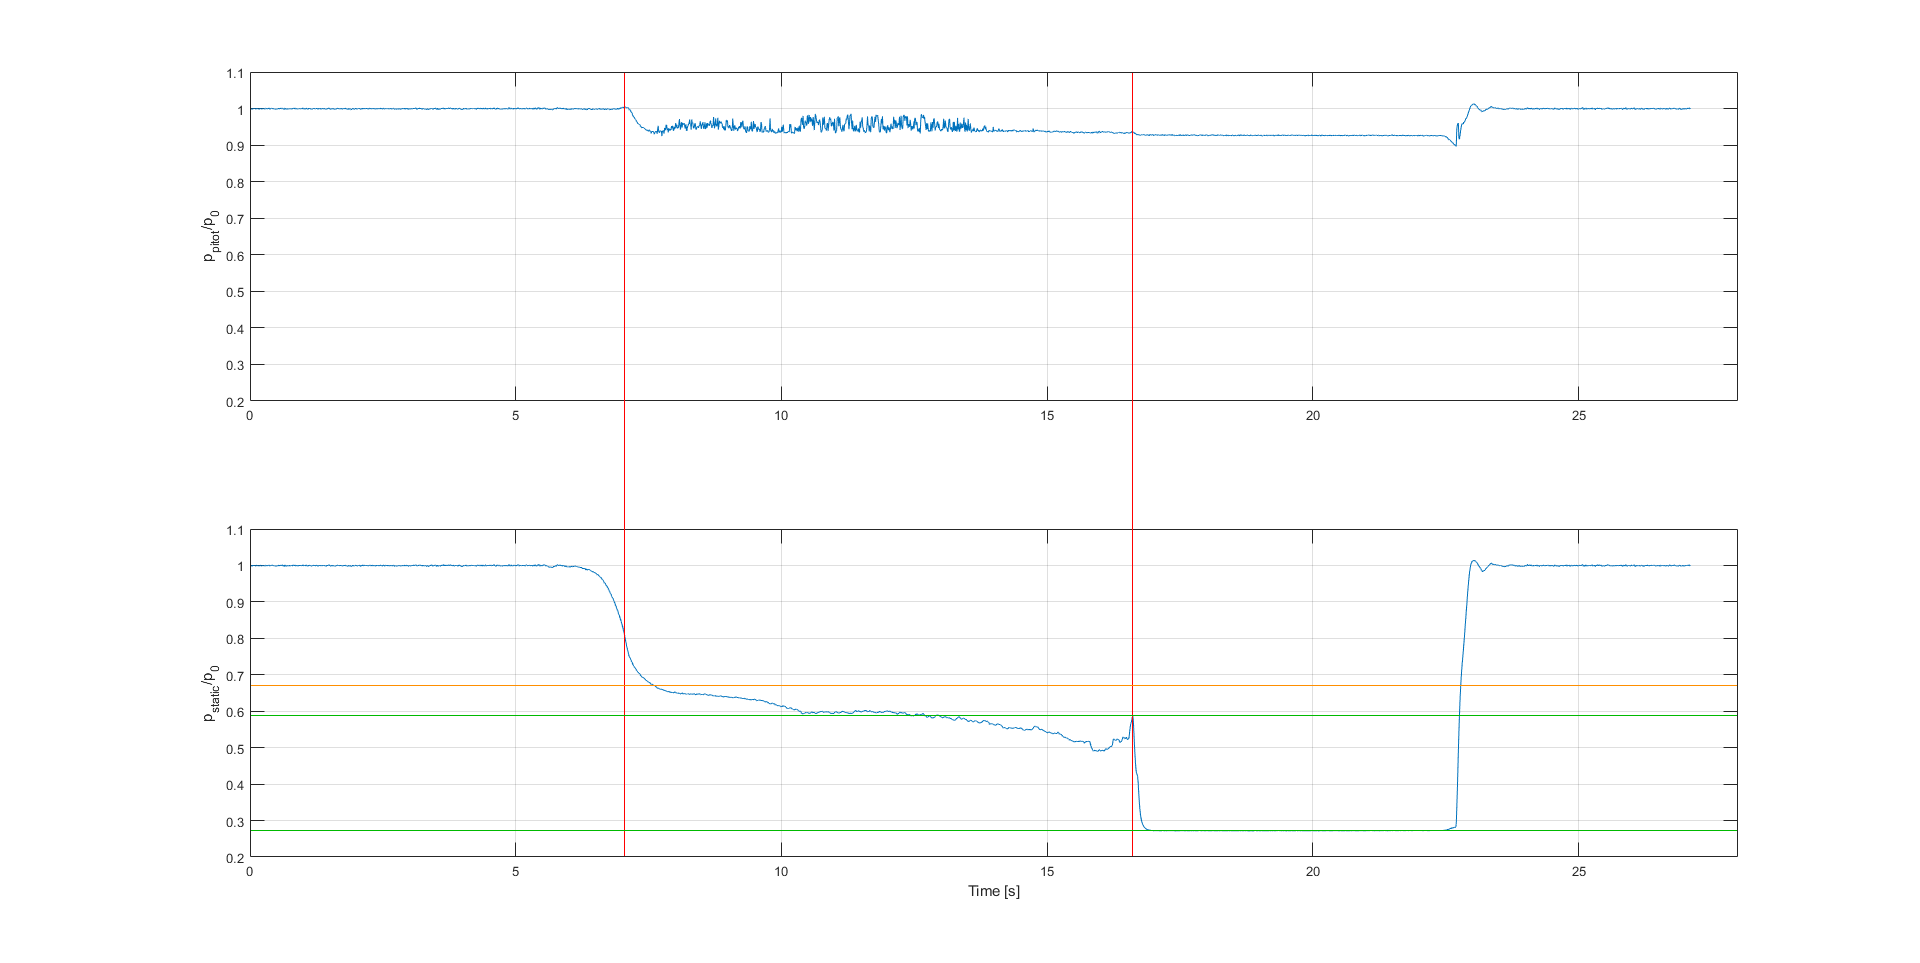
\includegraphics[width=1\textwidth]{tunnel_pressures_annotated.png}
    \caption{Annotated readings of the pressure sensors over time during the experiment. Top graph shows the stagnation pressure ratio, and the bottom graph shows the static pressure ratio.}
    \label{fig:figure8}
\end{figure}

Figure \ref{fig:figure8} shows the annotated readings of the pressure sensors over time during the experiment.
It can be observed that before the first vertical red line, the static pressure decreases which corresponds to the subsonic flow accelerating.
At the red line the normal shock wave is formed upstream of the sensors, by the supersonic flow downstream of the throat.
The stagnation pressure readings then becomes very noisy as the shock wave moves further downstream (WHY?) Shock trains?.
The static pressure ratio slowly decreases indicating an acceleration in the flow, and then suddenly increases again indicating deceleration.
This may be due to the boundary layer growing and then shrinking rapidly as the shock wave moves closer to the sensors.

After the shock has passed, the green line shows a static pressure ratio of around 0.275. This corresponds to a Mach number of 1.49, which is very close to the set operating point of Mach 1.5.
The top green line shows the static pressure ratio of the flow before the shock at 0.59.


\end{document}
